\chapter{序論}
\label{chap_Introduction}

XXXXXXXXXXXXXXXXX序論

\section{先行研究}
ハッシュテーブルの実実装の内,
探査の高速な実装として google::dense\_hash\_map (以下 dense\_hash\_map) が知られている.
dense\_hash\_map はスループットで 250 query/$\mu$s 程度
\footnote{AMD Ryzen7 1700 (8C/16T) 3.7 GHz の場合.詳細は,第\ref{chap_Results}章を参照.}
の探査速度を持つことから,
探査 1 回の実行時間は 4 ns
\footnote{
  \begin{align*}
    250{\rm [query \slash \mu s]}
    = \frac{1}{250} {\rm [\mu s \slash query]}
    = \frac{10^3}{250} {\rm [ns \slash query]}
    = 4 {\rm [ns \slash query]}
  \end{align*}
}
である.このとき,3.7 GHz の CPU では単位 clock あたりの実行時間が,
$2.7 \times 10^{-1}$ [ns/clock]
\footnote{
  \begin{align*}
    \frac{1}{3.7 {\rm [GHz]}}
    = \frac{1}{3.7 \times 10^9}{\rm [sec]}
    = 2.7 \times 10^{-10}{\rm [sec]}
    = 2.7 \times 10^{-1}{\rm [ns/clock]}
  \end{align*}
}
となる.したがって,探査 1 回に必要な CPU cycle は
15 clock 程度
\footnote{
  \begin{align*}
    \frac{ 4 {\rm [ns/query]} }{ 2.7 \times 10^{-1} {\rm [ns/clock]} }
    = \frac{ 4 }{ 2.7 \times 10^{-1} } {\rm [clock/query]}
    \simeq 15 {\rm [clock/query]}
  \end{align*}
}
である.




探査の高速なハッシュテーブルアルゴリズムには,



探査の高速なハッシュテーブルアルゴリズムには,
キャッシュミスの少ない Closed hashing が上げられる.
1) Linear probing と 2) Quadratic probing は,
Closed hashing の主要なハッシュ値の衝突解決アルゴリズムである.
1) は,

メモリ
.

%\begin{figure} % 特に強い理由がない限り、[htbp]のような指定はしないでください。
%  \centering
%  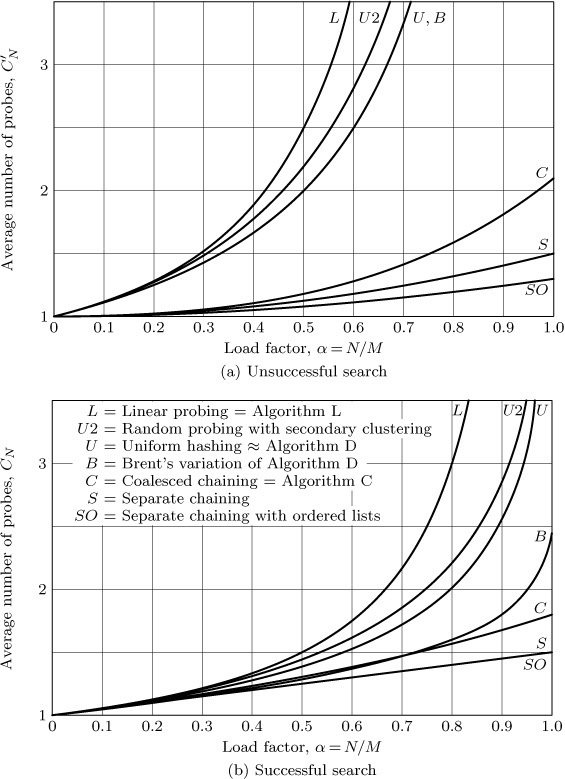
\includegraphics[width=10cm]{./figs/taocp_v3_fig44.png}
%  \caption{
%    Comparison of collision resolution methods: limiting values of the average number of probes as $M \rightarrow \infty$ \citep{knuth1998}.
%  }
%  \label{fig_taocp_v3_fig44}
%\end{figure}

%先行研究\footnote{脚注はこのように挿入します.}.


\section{Purpose}
研究目的.

